\documentclass{beamer}
\usetheme{Goettingen}
\usecolortheme{orchid}
\usefonttheme{structuresmallcapsserif}
\usepackage[utf8]{inputenc}
\usepackage{hyperref}


\graphicspath{'X:/Users/Josh/Dropbox/poker/DC/3BP/Higher Level/Why we 3-bet/Isolate.png'}
%Information to be included in the title page:
\title{Why do we 3-bet?}
\subtitle{Part of a Comprehensive Guide to All Things Related to 3-Bets}
\author{Josh Plotkin}
\institute{DeucesCracked.com}
\date{}

\AtBeginSection[]
{
  \begin{frame}
    \frametitle{Video Overview}
    \tableofcontents[currentsection,currentsubsection]
  \end{frame}
}

\begin{document}

\frame{\titlepage}

\section{Outline}
\begin{frame}
\begin{itemize}
\frametitle{Outline}
\item The Tree
\pause
\item Why I'm Trying this
\pause
\item How I Plan To Do This
\pause
\end{itemize}
\end{frame}

\section{The Tree}
\begin{frame}
\frametitle{The Tree}
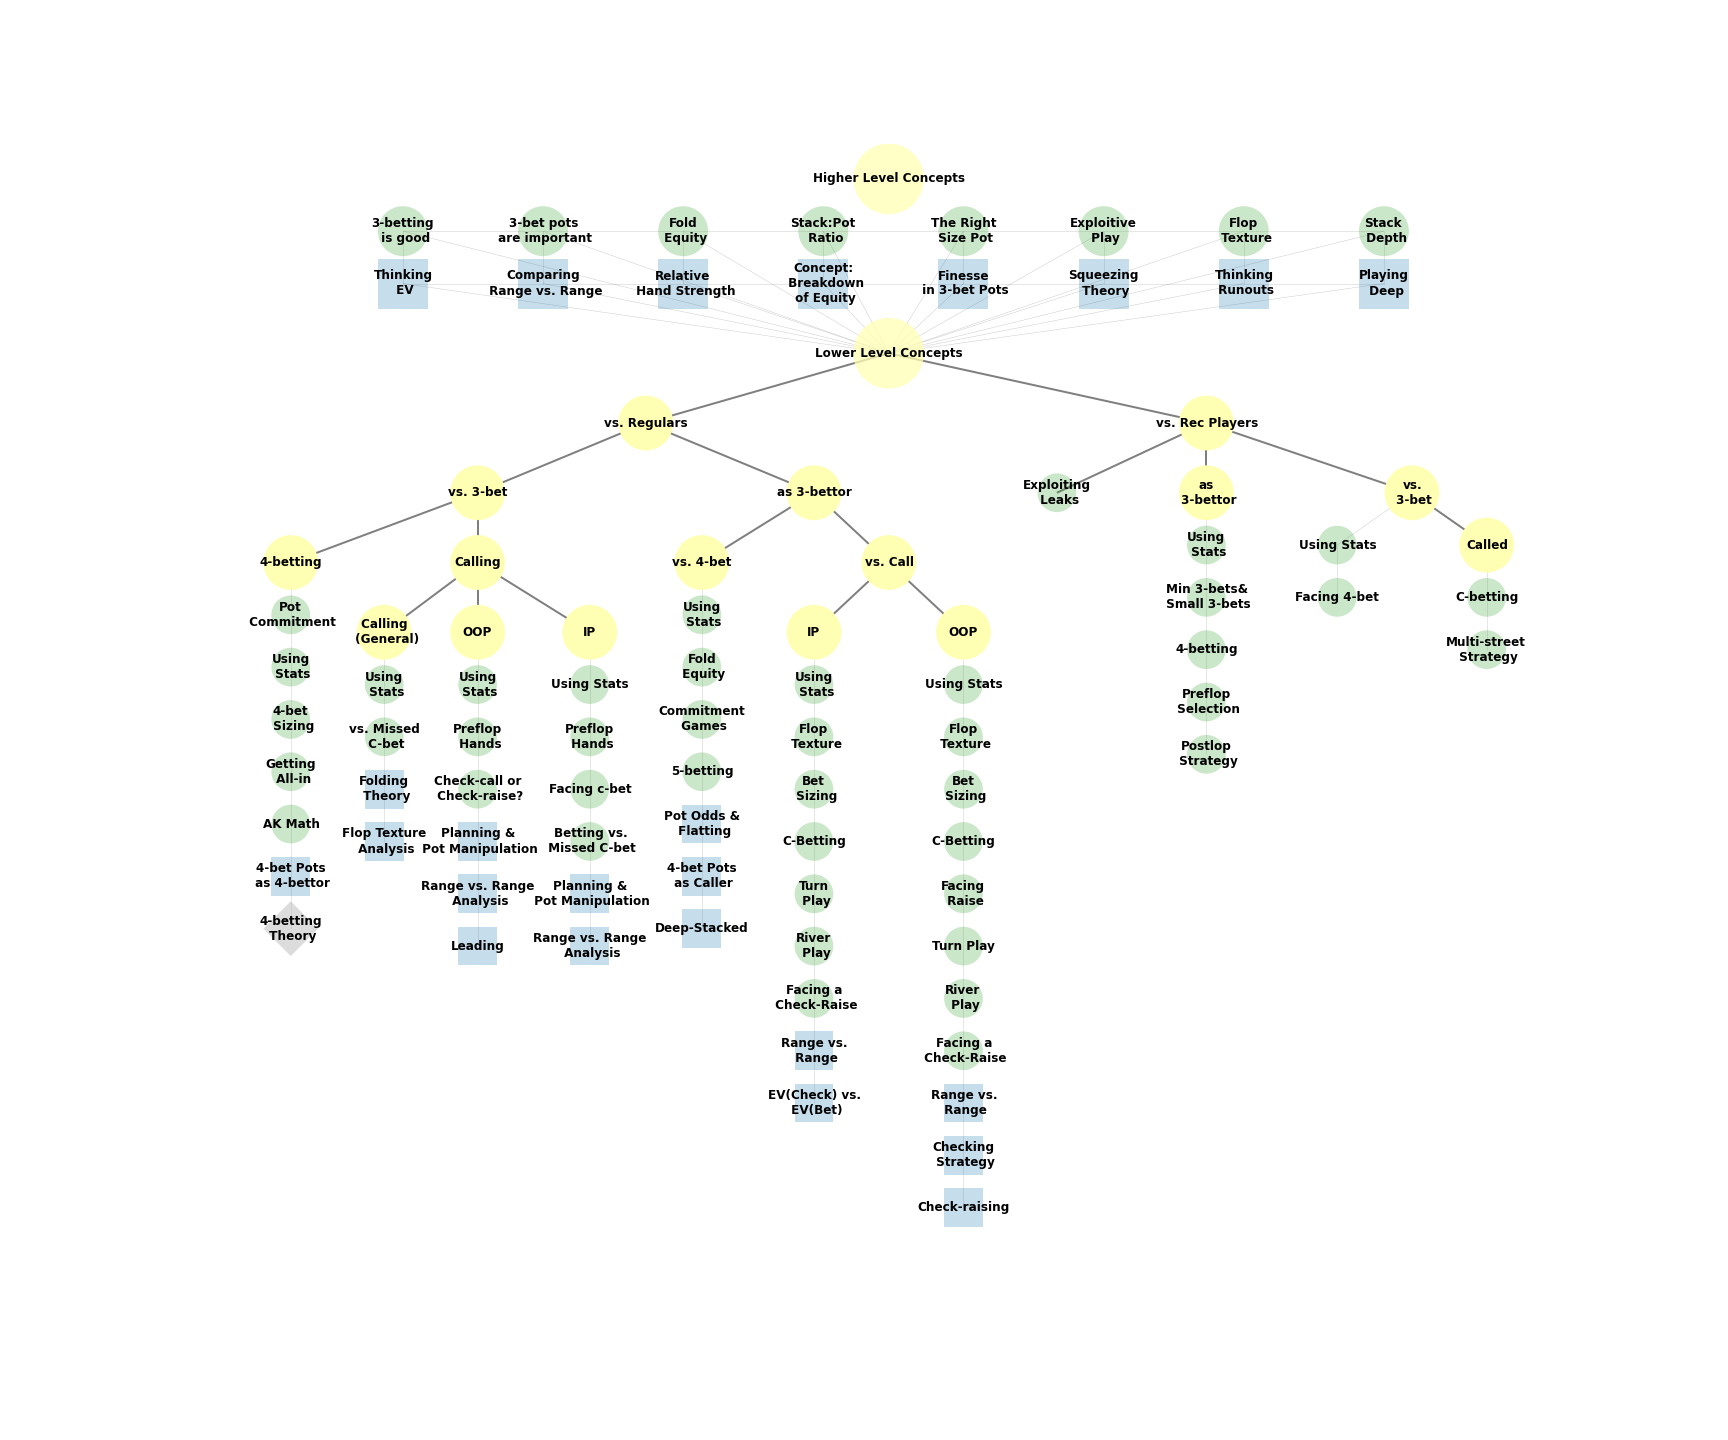
\includegraphics[keepaspectratio=true,width=.8\paperwidth]{InitialTree/tree.png}

\end{frame}

%\subsection{More basics}

\section{Why I'm Trying this}
\begin{frame}
\frametitle{Why I'm Trying this}
\begin{itemize}
\item Status of the 8-video Series
\item Series are Linear
\item A Set Path
\item Focused Videos
\item Variable Difficulty
\item Freedom to choose topics
\end{itemize}
\end{frame}

\section{How I Plan To Do This}
\begin{frame}
\frametitle{How I Plan To Do This}
\begin{itemize}
\item No set schedule
\item Others can join
\item Homework/Quizzes
\item Open Source
\item \url{https://github.com/joshplotkin/3BP}
\end{itemize}
\end{frame}

\end{document}

